\section{基本块分解与第一种证明}\label{sec:blocks}

\subsection{列切口的完整状态规则}
先考虑任意宽度 $w$ 的三行棋盘。在第 $j$ 列与第 $j+1$ 列之间记
$S_j\subseteq\{1,2,3\}$ 为被水平砖跨越的行集合，端点取
$S_0=S_w=\varnothing$。
若一列的输入和输出状态分别为 $p,q$，则合法的充要条件为
\begin{equation}\label{eq:local3}
 p\cap q=\varnothing,\qquad
 \{1,2,3\}\setminus(p\cup q)\in
 \{\varnothing,\{1,2\},\{2,3\}\}.
\end{equation}
理由是输入行的格已被左来的砖占用，输出行用于向右的砖，其余格必须在本列用竖直砖配对。
每个合法转移的本列填充唯一。全部转移见表 \ref{tab:states}。

\begin{table}[htbp]
\centering
\caption{三行的完整列状态转移。}\label{tab:states}
\begin{tabular}{cc@{\qquad}cc}
\toprule
输入 & 全部输出 & 输入 & 全部输出\\
\midrule
$\varnothing$ & $\{1\},\{3\},\{1,2,3\}$ &
$\{1,2\}$ & $\{3\}$\\
$\{1\}$ & $\varnothing,\{2,3\}$ &
$\{1,3\}$ & $\{2\}$\\
$\{2\}$ & $\{1,3\}$ &
$\{2,3\}$ & $\{1\}$\\
$\{3\}$ & $\varnothing,\{1,2\}$ &
$\{1,2,3\}$ & $\varnothing$\\
\bottomrule
\end{tabular}
\end{table}

\begin{lemma}\label{lem:path}
三行、$w$ 列的完整铺法与表 \ref{tab:states} 中长度为 $w$、
从空状态回到空状态的合法路径一一对应。
\end{lemma}
\begin{proof}
铺法唯一确定各切口状态。反过来，在每个切口状态指定的行放跨切口水平砖，
再在每列剩余行放唯一的竖直砖。式 \eqref{eq:local3} 保证同格不被两个水平砖重复使用，
且剩余格恰好被竖直砖覆盖。端点空状态排除越界砖。
两种构造互逆；$w=0$ 对应空路径。
\end{proof}

\subsection{首次回返路径与不可竖切块}
\begin{definition}
若一个内部竖直格线没有砖跨越，称它为断口。
非空完整铺法若没有内部断口，称为基本块。
\end{definition}

\begin{lemma}[基本块分类]\label{lem:blocks}
所有三行基本块恰为 $C$ 及 $A_k,B_k$（$k\ge1$）。
其中 $C$ 为宽 2 的三块水平砖；$A_k$ 宽 $2k$，由下列砖组成：
\begin{enumerate}
\item 第 1 列和第 $2k$ 列各放一块覆盖第 1、2 行的竖直砖；
\item 第 3 行按列对 $(2j-1,2j)$ 铺满，$1\le j\le k$；
\item 第 1、2 行内部各按列对 $(2j,2j+1)$ 铺满，$1\le j<k$。
\end{enumerate}
最后令 $B_k=h(A_k)$。
\end{lemma}
\begin{proof}
基本块对应空状态的首次回返路径。从空状态出发只有三个分支。
若第一步到 $\{1,2,3\}$，下一步被迫回空状态，给出 $C$。
若第一步到 $\{3\}$，则在最终回空状态之前，
只能在 $\{3\}$ 与 $\{1,2\}$ 之间交替。路径恰为
\[
 \varnothing\longrightarrow\{3\}
 \longrightarrow
 \bigl(\{1,2\}\longrightarrow\{3\}\bigr)^{k-1}
 \longrightarrow\varnothing,\qquad k\ge1,
\]
这里括号内表示两步的重复，$k=1$ 时重复零次。
路径给出所述 $A_k$ 坐标。第一步到 $\{1\}$ 的分支
只能在 $\{1\},\{2,3\}$ 之间交替后回空状态，得到 $B_k$。
表 \ref{tab:states} 穷尽了这些分支的所有后继，因而无遗漏。
$A_k$ 的奇数内部切口由第 3 行水平砖跨越，
偶数内部切口由第 1、2 行水平砖跨越，故确实无断口；
$B_k$ 由反射得到同样性质。
首列的竖直砖位置区分 $A_k,B_k$，而 $C$ 无竖直砖，故无重计。
\end{proof}

\begin{figure}[htbp]
\centering
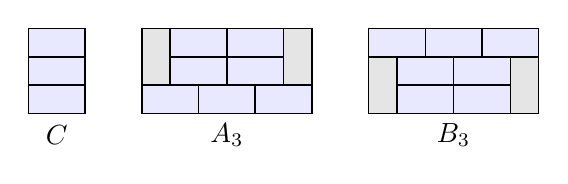
\begin{tikzpicture}[x=0.36cm,y=0.36cm,line width=0.55pt]
\begin{scope}
 \foreach \y in {0,1,2}{\draw[fill=blue!9] (0,\y) rectangle ++(2,1);}
 \node at (1,-0.75) {$C$};
\end{scope}
\begin{scope}[shift={(4,0)}]
 \draw[fill=gray!20] (0,1) rectangle (1,3);
 \draw[fill=gray!20] (5,1) rectangle (6,3);
 \foreach \x in {0,2,4}{\draw[fill=blue!9] (\x,0) rectangle ++(2,1);}
 \foreach \y in {1,2}{\foreach \x in {1,3}{\draw[fill=blue!9] (\x,\y) rectangle ++(2,1);}}
 \node at (3,-0.75) {$A_3$};
\end{scope}
\begin{scope}[shift={(12,0)}]
 \draw[fill=gray!20] (0,0) rectangle (1,2);
 \draw[fill=gray!20] (5,0) rectangle (6,2);
 \foreach \x in {0,2,4}{\draw[fill=blue!9] (\x,2) rectangle ++(2,1);}
 \foreach \y in {0,1}{\foreach \x in {1,3}{\draw[fill=blue!9] (\x,\y) rectangle ++(2,1);}}
 \node at (3,-0.75) {$B_3$};
\end{scope}
\end{tikzpicture}

\caption{三种基本块的代表 $C,A_3,B_3$。矩形边界表示实际砖界；图示不代替一般分类证明。}
\label{fig:blocks}
\end{figure}

\begin{lemma}[唯一块分解及对称作用]\label{lem:word}
每个完整三行铺法唯一对应基本块字母表
$\mathcal B=\{C\}\cup\{A_k,B_k:k\ge1\}$ 上的一个有限字。
令 $\sigma$ 固定 $C$，交换 $A_k$ 与 $B_k$，则字上的作用为
\begin{equation}\label{eq:word-action}
 h(W)=\sigma(W),\qquad v(W)=\rev(W),\qquad
 \rho(W)=\sigma(\rev(W)).
\end{equation}
\end{lemma}
\begin{proof}
沿全部断口切开，所得各段无内部断口，故由引理 \ref{lem:blocks} 都是基本块。
任何基本块分解的分界必须是断口，而且不能遗漏断口，
否则有一块内部仍可竖切。这证明唯一性。任意基本块字的拼接给出逆映射。

上下反射在各块内按定义施加 $\sigma$。每个基本块还都左右对称：
对 $A_k$，列反转 $c\mapsto2k+1-c$ 交换两端竖直砖，
将底行列对 $(2j-1,2j)$ 映为同类列对，
将上两行列对 $(2j,2j+1)$ 映为同类列对；
对应指标分别为 $k+1-j$ 和 $k-j$。$C$ 逐砖不变。
由于上下、左右反射交换，$B_k=h(A_k)$ 也左右对称。

全棋盘反射保持断口集合；上下反射保留块次序，
左右反射颠倒块次序。结合唯一分解即得 \eqref{eq:word-action}。
论证允许相邻块宽度不同。
\end{proof}

\subsection{固定字的生成函数}
给 $C$ 权 $x$，给 $A_k,B_k$ 权 $x^k$，权的指数为半长度。
基本块生成函数为
\begin{equation}\label{eq:F}
 F(x)=x+2\sum_{k\ge1}x^k=\frac{3x-x^2}{1-x}.
\end{equation}
由于 $F(0)=0$，每个次数只涉及有限多个字，形式求和合法。

\begin{proposition}\label{prop:fixed-gf}
四种固定点生成函数为
\begin{align}
D(x)&=\frac{1}{1-F(x)}=\frac{1-x}{1-4x+x^2},&
H(x)&=\frac{1}{1-x},\label{eq:DH}\\
V(x)&=(1+F(x))D(x^2)
 =\frac{1+3x+x^2-x^3}{1-4x^2+x^4},\label{eq:V}\\
R(x)&=(1+x)D(x^2)
 =\frac{1+x-x^2-x^3}{1-4x^2+x^4}.\label{eq:R}
\end{align}
\end{proposition}
\begin{proof}
普通铺法对应任意字，故 $D=\sum_{\ell\ge0}F^\ell$。
上下反射固定字的每个字母须由 $\sigma$ 固定，唯一选择为 $C$，
故 $H=\sum_{\ell\ge0}x^\ell$。

左右反射固定字是回文，唯一写为
$U\rev(U)$ 或 $Ub\rev(U)$，其中 $b$ 为任意基本块。
两侧的总权是左侧权的平方，所以左半字贡献 $D(x^2)$，
中间贡献 $1+F(x)$，得到 \eqref{eq:V}。

半周旋转固定字唯一写为
$U\sigma(\rev(U))$，或 $Ub\sigma(\rev(U))$ 且 $\sigma(b)=b$。
后一种情形只允许 $b=C$，故中心贡献 $1+x$。
这两类互斥，分解可逆，得到 \eqref{eq:R}。
中心基本块允许跨越几何中线；上述计数没有附加中线必须为断口的限制。
\end{proof}

\begin{proof}[定理 \ref{thm:main} 的第一种证明]
由引理 \ref{lem:burnside} 和命题 \ref{prop:fixed-gf}，
\begin{equation}\label{eq:average-rational}
 A(x)=\frac14\left[
 \frac{1-x}{1-4x+x^2}+\frac1{1-x}
 +\frac{2(1+2x-x^3)}{1-4x^2+x^4}\right].
\end{equation}
记 $P_3=1-4x+x^2$、$Q_3=1-4x^2+x^4$。
通分后分子为
\[
 \frac{(1-x)^2Q_3+P_3Q_3+
 2(1+2x-x^3)(1-x)P_3}{4}
 =1-3x-4x^2+10x^3-4x^5+x^6.
\]
这给出 \eqref{eq:main}。分母展开为
\[
 1-5x+x^2+19x^3-19x^4-x^5+5x^6-x^7.
\]
因分子次数为 6，比较次数 $n\ge7$ 的系数得到
\eqref{eq:recurrence}；比较次数 $0,\ldots,6$ 得到所述初值。
\end{proof}

Mathar \cite[式 (26)]{mathar2013} 以全列数为指数，故与本文比较应取
$\overline T(z,3)=A(z^2)$。将 $x=z^2$ 代入
\eqref{eq:average-rational}，其中上下反射项重排利用
$\tfrac18((1+z)^{-1}+(1-z)^{-1})=(4(1-z^2))^{-1}$，
即得到该文献的表达式。
Mathar \cite[式 (4)--(6)]{mathar2014} 的三行公式以砖数计次，
对应换元为 $z^3=x$。两种变量约定不可混用。
